\section{How Often Channels Force-Close}
\label{sec:census}

\begin{table*}[t]
\centering
\caption{Lightning channel closes on the chain, 2018--2026. All force: every force close, public or not. Public: channels in our list of every public channel. Unlisted: force closes of channels outside it, found by the commitment pattern.}
\label{tab:census}
\footnotesize
\begin{tabular}{lrrrrrrrrrr}
\toprule
Year & All force & Coop. & Force & Force \% & Force BTC & Age (d) & Unlisted & Unl. BTC & Pub. legacy \% & Unl. taproot \% \\
\midrule
2018\textsuperscript{b} & 35{,}218 & -- & -- & -- & -- & -- & -- & -- & -- & -- \\
2019\textsuperscript{c} & 52{,}148 & 30{,}404 & 30{,}001 & 49.7 & 679 & 80 & 22{,}147 & 411 & 100.0 & 0.0 \\
2020 & 29{,}877 & 28{,}785 & 17{,}813 & 38.2 & 581 & 159 & 12{,}064 & 198 & 100.0 & 0.0 \\
2021 & 39{,}539 & 64{,}048 & 27{,}393 & 30.0 & 1{,}123 & 94 & 12{,}146 & 179 & 87.5 & 0.0 \\
2022 & 73{,}569 & 92{,}645 & 57{,}896 & 38.5 & 3{,}226 & 133 & 15{,}673 & 264 & 44.8 & 0.0 \\
2023 & 76{,}869 & 62{,}481 & 49{,}998 & 44.5 & 3{,}363 & 151 & 26{,}871 & 764 & 40.2 & 0.1 \\
2024 & 76{,}634 & 50{,}874 & 28{,}888 & 36.2 & 2{,}208 & 215 & 47{,}746 & 1{,}410 & 33.9 & 0.6 \\
2025 & 71{,}498 & 58{,}137 & 21{,}518 & 27.0 & 1{,}975 & 242 & 49{,}980 & 838 & 23.4 & 3.2 \\
2026\textsuperscript{a} & 68{,}463 & 62{,}311 & 15{,}440 & 19.9 & 2{,}279 & 142 & 53{,}023 & 974 & 25.6 & 23.1 \\
\bottomrule
\end{tabular}
\par\smallskip\parbox{\linewidth}{\scriptsize \textsuperscript{a}January--October. \textsuperscript{b}From 12 January (block 503,816). Our list of public channels holds few of the channels that closed in 2018, so only the force-close total is shown. \textsuperscript{c}The list's coverage is still ramping up in January 2019. Age: median age at force close. Pub.\ legacy: share of public force closes with a pre-anchor commitment. Unl.\ taproot: share of unlisted force closes of simple taproot channels. Splices (59) are not shown.}
\end{table*}


\begin{figure*}[t]
\centering
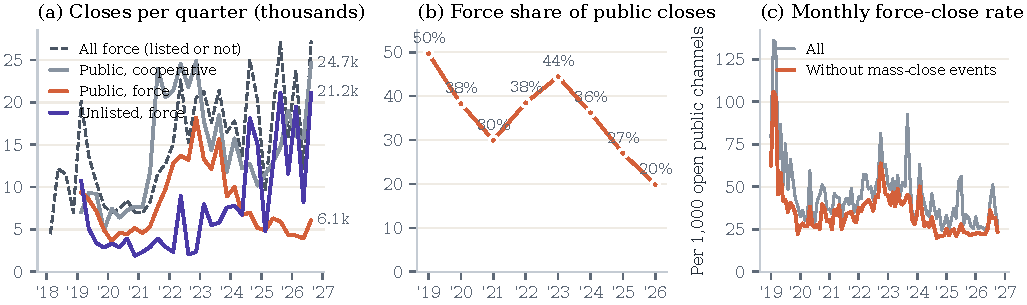
\includegraphics[width=\textwidth]{figures/fig1_census.pdf}
\caption{Lightning channel closes on the chain. (a) Closes per quarter: all force closes, listed or not (dashed,
from January~2018), and from 2019 the cooperative and force closes of public channels and the force closes of
channels outside our list of public channels (unlisted). (b) Force share of public closes by year, from 2019.
(c) Public force closes per 1,000 open public channels per month, from 2019, with and without mass-close events
(one node party to at least \MassMin{} force closes on one UTC day).}
\label{fig:census}
\end{figure*}

\paragraph{Force closes became rarer, but less than their counts suggest}
Public force closes peaked at \PubForceTwentyTwo{} in 2022 and fell to \PubForceTwentySix{} in the first ten months of
2026 (Table~\ref{tab:census}). Part of that fall is a smaller network: open public channels peaked at \OpenPeak{} and
stood at \OpenAtCutoff{} at the cutoff. Part is more cooperative closing: cooperative closes released
\MutualBtcTwentyFour~BTC of capacity in 2024 and \MutualBtcTwentyFive~BTC in 2025. The force share of public closes
therefore fell faster than the risk to a channel. It went from \ForceShareTwentyThree\% in 2023 to
\ForceShareTwentySix\% in 2026, while the organic force-close rate went from \OrganicRateTwentyThree{} to
\OrganicRateTwentySix{} per 1,000 open channels a month (Fig.~\ref{fig:census}c).

\paragraph{2019 reads highest, but our list may be incomplete}
In 2019 the force share (\ForceShareNineteen\%) and the organic rate (\OrganicRateNineteen{} per 1,000 open channels a month)
were the highest of any year. We do not read this as a peak, because our channel list may still have been filling in. In
February and March~2019 the organic rate was \RateOrganicFebNineteen{} and \RateOrganicMarNineteen{} per 1,000, and
no later month exceeded \RateOrganicMaxLater.

\paragraph{The risk to a new channel fell}
\CohortOneYearNineteen\% of the public channels funded in 2019 were force-closed within a year, against
\CohortOneYearTwentyFive\% of those funded in 2025 (Fig.~\ref{fig:cohorts}). The fall was not steady: the share
dropped to \CohortOneYearTwentyOne\% for the 2021 cohort, rose to \CohortOneYearTwentyThree\% for 2023's and fell
again after. Cohort incidence does not depend on the count of open channels, which abandoned channels inflate, so it
is the cleaner measure of the trend.

\begin{figure}[t]
\centering
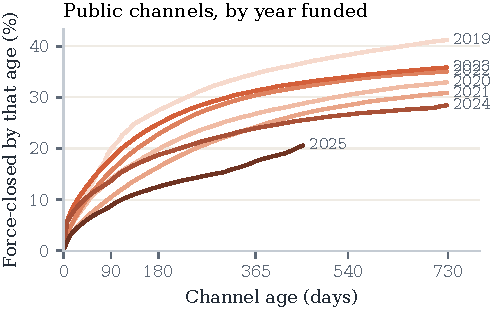
\includegraphics[width=\columnwidth]{figures/fig2_cohorts.pdf}
\caption{Share of public channels force-closed by each channel age, by the year the channel was funded (2019--2025).
A curve ends where less than half of its cohort has been observed for that long.}
\label{fig:cohorts}
\end{figure}

\paragraph{Much force closing is one node closing many channels at once}
Every year has \MassEventsMin--\MassEventsMax{} mass-close events, which hold \MassShareMin--\MassShareMax\% of public
force closes; the largest put \MassLargest{} channels on-chain in one day. Without them the rate still falls, so the
decline is not one operator's. The 2026 peak is such an episode. In August~2026 the rate reached \RateAugTwentySix{}
per 1,000 open channels, \RateOrganicAugTwentySix{} without mass-close events, while open channels fell from
\OpenJulTwentySix{} in July to \OpenAtCutoff{} at the cutoff. That month brought the Core Lightning shutdown and the
largest contraction of the public graph. Our first paper found the contraction driven by large operators leaving,
and organic force closes of channels with a Core Lightning node above their usual rate after the
shutdown~\cite{kumar2026clientdiversity}.

\paragraph{Most force closes now happen outside the public network}
In 2026, unlisted force closes outnumbered public ones \UnlOverPubTwentySix{} to one. From 2024 on they are almost all
private channels; before 2024 they include public channels missing from our list (\S\ref{sec:limitations}).
Private channels are often those of mobile wallets~\cite{bitmex2020closures}, and \UnlTaprootPctTwentySix\% of
2026's unlisted force closes were simple taproot channels. The largest burst in the data is unlisted: on 1~September~2024, \SepEventCloses{} unlisted force closes
holding \SepEventBtc~BTC confirmed within about \SepEventHours~hours (\SepEventBlocks{} blocks), \SepEventLegacy{} of
them pre-anchor.

\paragraph{Most of 2026's pre-anchor closes are one cluster}
Pre-anchor commitments were \PubLegacyPctTwentyOne\% of public force closes in 2021 and \PubLegacyPctTwentySix\% in
2026 (Table~\ref{tab:census}), but most of the 2026 share is one cluster. Five nodes were party to
\LegacyTopFivePct\% of 2026's pre-anchor public force closes, four of them LDK nodes that announced no anchor
support~\cite{kumar2026clientdiversity}, and their channels lasted a median of \LegacyClusterAgeDays~days. Without
closes involving those nodes, pre-anchor commitments were \LegacyPctExClusterTwentySix\% of 2026 public force closes,
and those channels were old (median \LegacyOldAgeYears~years).

\paragraph{Client pairs}
Among client pairs with more than 1,000 closes since May~2023, the force share ranges from \PairForcePctLndLnd\%
(LND--LND) to \PairForcePctClnCln\% (CLN--CLN), with one outlier that a single node explains
(Appendix~\ref{app:pairs}; labels from~\cite{kumar2026clientdiversity}).
